\chapter{Elaboration of the Workflow}
\label{chapter:elaboration}

This chapter details the implementation of the analyses and the additional proceedings about analysing more than one \es modules coherently. Thus, this chapter encompasses all \emph{semantic} changes of the framework.

Following Dániel Stein~\cite{stein-daniel-msc} and \Cref{chapter:overview} of this thesis, a full analysis procedure of the Codemodel-Rifle framework can be broken down to three distinct phases:

\begin{enumerate}
\item \textsc{\textbf{Import:}} The analysed code repository's \es source files (meaning \es \emph{modules}) are imported into Codemodel-Rifle. After parsing the modules, they get translated to Abstract Semantic Graph models. The ASGs are stored as distinct, per-module property graphs in the underlying Neo4j graph database.
\item \textsc{\textbf{Interconnect:}} The related modules' separate graphs are interconnected along the \emph{export} and \emph{import} semantics of \es. This makes possible to evaluate analyses over more than one modules coherently.
\item \textsc{\textbf{Analyse:}} The predefined analyses are executed.
	\begin{enumerate}
	\item The necessary graph manipulations of the \emph{Qualifier System} are performed.
	\item The defect patterns are matched.
	\end{enumerate}
\end{enumerate}

Since I have not made any semantic changes to the \textsc{Import} phase, this chapter focuses to the \textsc{Interconnect} and the \textsc{Analyse} phases.


\section{Interconnecting Related \es Modules}

This section describes the work I made to support analysing more than one \es modules coherently. The approach follows~\cite{stein-daniel-msc}, and completes it by implementing missing use cases. To shorty summarise: in order to coherently analyse several related \es modules with the Codemodel-Rifle framework, the related modules' separate property graphs are interconnected by well-defined rules. As previously already mentioned, these rules are built upon the \emph{export} and \emph{import} semantics of \es~\cite{exploringes6}. Equivalently, \es modules are considered to be \emph{related}, if they refer to each other by using \emph{export} and \emph{import} statements.


\subsection{The \es Module System}

As the language gained traction, JavaScript projects rapidly grown to a size where modularisation became critical in order to keep the code logically organised. Today's largest \es code bases include Google's Gmail\footnote{\texttt{https://www.gmail.com}} with approx. 400,000 lines of code~\cite{gmail-loc}, Ruben Daniels' Cloud9 IDE\footnote{\texttt{https://c9.io}} with approx. 300,000 lines of code~\cite{cloud9-loc}, and Lucidchart\footnote{\texttt{https://www.lucidchart.com}} with approx. 200,000 lines of code~\cite{lucidchart-loc}. The product of Tresorit featured in this thesis consists of approx. 35,000 lines of \es code.

Plain JavaScript does not have built-in support for modules~\cite{exploringes6}, there are only community-provided solutions like \emph{RequireJS}\footnote{\texttt{http://requirejs.org}}. In contrary, the 6\textsuperscript{th} version of \es has language-level support for modules: each source file represents exactly one module. Entities like variables and functions defined in one module, or even complete modules themselves can be \emph{exported} to be later \emph{imported} to a different module. By default, modules are referred by their relative pathname, without the file extension. Entities that are not exported remain \emph{private}, meaning they can not be imported to other modules.

In \es 6, there are several ways of exporting and importing entities~\cite{exploringes6}, these are detailed in the next subsections. The Codemodel-Rifle framework had only minimal demonstrative support for interconnecting several \es modules; I extended Dániel Stein's work by covering the most used \emph{export-import cases}.


\subsection{Export Syntaxes and Cases}

By default, each entity can only be accessed in the scope of the module it was declared in. To be accessed from other modules, the entity has to be explicitly exported first. \Cref{fig:export-syntaxes} presents export syntax examples of \es 6, based on~\cite{export-syntaxes}. Since these statements can be almost arbitrarily combined, and the number of exported variables is not limited in theory, the list of differing export syntaxes of \es 6 is practically endless.

Therefore, \emph{export syntaxes} need to be distinguished from \emph{export cases}. An \emph{export case} is identified by the \emph{basic form} of an \emph{export syntax}. An \emph{export syntax} written in \emph{basic form} does not combine divers syntaxes, and exports only one entity per export statement. \Cref{fig:export-syntaxes} displays all syntaxes in \emph{basic form}, thus it lists all members of the \emph{export cases'} finite set. Each different \emph{export case} represents a unique graph pattern in the ASG.

\begin{figure}[!p]
	\centering
	\begin{lstlisting}[language=JavaScript]
			// exportName
			export { name1, ... };
			// exportDefaultName
			export default name1;
			// exportAlias
			export { name1 as exportedName1, ... };
			// exportAsDefault
			export { name1 as default, ... };
			// exportEmptyLetDeclaration
			export let name1, ... ;
			// exportEmptyVarDeclaration
			export var name1, ... ;
			// exportLetDeclaration
			export let name1 = ..., ... ;
			// exportVarDeclaration
			export var name1 = ..., ... ;
			// exportConstDeclaration
			export const name1 = ..., ... ;
			// exportClass
			export class name1 { ... }
			// exportFunction
			export function name1(...) { ... }
			// exportGenerator
			export function* name1(...) { ... }
			// exportDefaultExpression
			export default expression;
			// exportDefaultAnonymousClass
			export default class { ... }
			// exportDefaultAnonymousFunction
			export default function (...) { ... }
			// exportDefaultAnonymousGenerator
			export default function* (...) { ... }
			// exportDefaultClass
			export default class name1 { ... }
			// exportDefaultFunction
			export default function name1(...) { ... }
			// exportDefaultGenerator
			export default function* name1(...) { ... }
			// exportExpression
			export expression;
			// reexportNamespace
			export * from ...;
			// reexportName
			export { name1, ... } from ... ;
			// reexportAlias
			export { import1 as importedName1, ... } from ...;
	\end{lstlisting}
  \caption{Export syntax examples of \es 6}
  \label{fig:export-syntaxes}
\end{figure}


\subsection{Import Syntaxes and Cases}

An entity declared in module \textbf{A} can be accessed in module \textbf{B}, if \textbf{A} exports, and \textbf{B} imports the entity. All exported entities of a module can be imported as well: in this case an object is created with the name of the imported module's alias, and with members listing the exported entities of the imported module. \Cref{fig:import-syntaxes} present import syntax examples of \es 6, based on~\cite{import-syntaxes}. Like the exports, these statements can also be combined with each other, making the list of the possible import syntax combinations endless.

Thus, \emph{import syntaxes} need to be distinguished from \emph{import cases}, similarly to the exports. An \emph{import case} is identified by the \emph{basic form} of an \emph{import syntax}. \Cref{fig:import-syntaxes} displays all syntaxes in \emph{basic form}. Each \emph{import case} has a unique graph pattern in the ASG.

\begin{figure}[!htb]
	\begin{lstlisting}[language=JavaScript]
		// importName
		import { name1, ... } from "exporter";
		// importAlias
		import { name1 as importedName1, ... } from "exporter";
		// importDefault
		import defaultName from "exporter";
		// importNamespace
		import * as exportedModule from "exporter";
		// importModule
		import "exporter";
	\end{lstlisting}
  \caption{Import syntax examples of \es 6}
  \label{fig:import-syntaxes}
\end{figure}


\subsection{Number of Export-Import Combinations}

Let $\mathbb{E}$ be the distinct export cases' set, and let $\mathbb{I}$ be the distinct import cases' set. As \Cref{fig:export-syntaxes} and \Cref{fig:import-syntaxes} show, $|\mathbb{E}| = 22$, and $|\mathbb{I}| = 5$. If all export cases would be compatible with all import cases according to the \es grammar, set $\mathbb{C}$ containing all combinations would be $\mathbb{C} = \mathbb{E} \times \mathbb{I}$ with the cardinality of $|\mathbb{C}| = |\mathbb{E}| * |\mathbb{I}| = 22 * 5 = 110$.

\begin{figure}[!htb]
	\begin{lstlisting}[language=JavaScript]
					// exporter.js
					export let name1 = ...;
					// importer.js
					import defaultName from "exporter";
	\end{lstlisting}
  \caption{An example of incompatible export-import cases}
  \label{fig:incompatible-export-import-example}
\end{figure}

Let $\mathbb{S}$ be the set of the export-import combinations supported by Codemodel-Rifle, and let $\alpha$ be the number of distinct algorithms needed to be implemented for supporting every element of $\mathbb{S}$. The following applies: $\alpha \leq |\mathbb{S}|$, since the framework needs one separate algorithm for each export-import case at most. Since not all export cases are compatible with all import cases (a counterexample is displayed on \Cref{fig:incompatible-export-import-example}), the set of \emph{semantically valid} export-import combinations is narrower than $\mathbb{C}$. Codemodel-Rifle should interconnect only semantically valid export-import cases, so $\mathbb{S} \subset \mathbb{C}$. Also, $\alpha$ can be reduced further by involving ASG-specific knowledge: with graph pattern generalisation techniques, several export cases can be handled as one at implementing the interconnections, while preserving semantics. Therefore several export cases can be covered by one algorithm, so $\alpha < |\mathbb{S}|$. In addition, by choosing particular export and import cases not to be supported by Codemodel-Rifle, $\alpha$ can be lowered even further. Case compatibility, unsupported cases and pattern generalisation techniques are detailed in the following subsections.


\subsection{Compatibility of the Export-Import Cases}

An export-import combination is considered to be \emph{semantically valid}, if it complies with the \es grammar~\cite{export-grammar, import-grammar}. Accordingly, semantically valid export-import combinations consist of \emph{compatible} export-import cases: export case \textbf{E} and import case \textbf{I} are considered to be \emph{compatible} with each other, if the entity exported by \textbf{E} can be imported by \textbf{I}, following the \es grammar. \Cref{fig:incompatible-export-import-example} shows an example of incompatible export-import cases. \Cref{table:export-import-compatibility} displays a compatibility matrix for \es export-import cases.

As only semantically valid export-import combinations are required to be supported by Codemodel-Rifle to evaluate analyses over several \es modules coherently, incompatible cases do not need to be covered. This reduces $\alpha$ from $110$ to $79$ (see \Cref{table:export-import-compatibility}).


\subsection{Unsupported Cases}

There are export and import cases which I chosen not be supported by Codemodel-Rifle because of implementation difficulties, or the cases' irrelevant usage. This reduces $\alpha$ from $79$ to $30$. The unsupported export and import cases are the following:

\begin{itemize}
\item \textbf{\lstinline{exportExpression}}: Unnamed expressions (e.g.\ \lstinline[language=JavaScript]{export 1 + 2;}) can not be imported, because they can not be referenced.
\item \textbf{\lstinline{exportDefaultExpression, exportDefaultAnonymousClass, export\- DefaultAnonymousFunction, exportDefaultAnonymousGenerator}}: There is no clear way for interconnecting the exported entities with the importer module.
\item \textbf{\lstinline{reexportName},} \textbf{\lstinline{reexportAlias},} \textbf{\lstinline{reexportNamespace}}: According to my experiences, re-exporting is used very little.
\item \textbf{\lstinline{importNamespace}}: There is no clear solution for including all exported variable of the imported module as an object into the ASG.
\item \textbf{\lstinline{importModule}}: It only loads the module, does not import anything. The first such import in a program executes the body of the module~\cite{exploringes6}.
\end{itemize}

\Cref{table:export-import-compatibility} displays unsupported export and import cases with a grey background. With excluding the incompatible and the unsupported cases from the interconnection process, $\alpha$ is reduced by more than $72\%$, from $110$ to $30$. This saves a significant amount of work without notable loss of the analyses' credibility — unsupported cases were mostly chosen because of their unpopularity. Nevertheless, these cases need to be covered later as well.

\begin{table}[!htb]
	\newcommand{\yep}{\tikz\draw[black,fill=black] (0,0) circle (0.8ex);\xspace}
	\newcommand{\nop}{\tikz\draw[black,fill=none] (0,0) circle (0.8ex);\xspace}

	\definecolor{grey}{gray}{0.85}
	\newcolumntype{g}{>{\columncolor{grey}}c}

	\small
	\centering
	\begin{tabular}{l|cccgg}
		\hline
																				& \rotatebox{90}{importName}
																				& \rotatebox{90}{importAlias}
																				& \rotatebox{90}{importDefault}
																				& \rotatebox{90}{importNamespace~~}
																				& \rotatebox{90}{importModule}
																				\\
		\hline
		{exportName}												& \yep & \yep & \nop & \yep & \yep \\
		{exportDefaultName}									& \yep & \yep & \yep & \yep & \yep \\
		{exportAlias}												& \yep & \yep & \nop & \yep & \yep \\
		{exportAsDefault}										& \nop & \nop & \yep & \nop & \yep \\
		{exportEmptyLetDeclaration}					& \yep & \yep & \nop & \yep & \yep \\
		{exportEmptyVarDeclaration}					& \yep & \yep & \nop & \yep & \yep \\
		{exportLetDeclaration}							& \yep & \yep & \nop & \yep & \yep \\
		{exportVarDeclaration}							& \yep & \yep & \nop & \yep & \yep \\
		{exportConstDeclaration}						& \yep & \yep & \nop & \yep & \yep \\
		{exportClass}												& \yep & \yep & \nop & \yep & \yep \\
		{exportFunction}										& \yep & \yep & \nop & \yep & \yep \\
		{exportGenerator}										& \yep & \yep & \nop & \yep & \yep \\
		{exportDefaultClass}								& \yep & \yep & \yep & \yep & \yep \\
		{exportDefaultFunction}							& \yep & \yep & \yep & \yep & \yep \\
		{exportDefaultGenerator}						& \yep & \yep & \yep & \yep & \yep \\
		\rowcolor{grey}
		{exportDefaultExpression}						& \nop & \nop & \yep & \nop & \yep \\
		\rowcolor{grey}
		{exportDefaultAnonymousClass}				& \nop & \nop & \yep & \nop & \yep \\
		\rowcolor{grey}
		{exportDefaultAnonymousFunction}		& \nop & \nop & \yep & \nop & \yep \\
		\rowcolor{grey}
		{exportDefaultAnonymousGenerator}		& \nop & \nop & \yep & \nop & \yep \\
		\rowcolor{grey}
		{exportExpression}									& \nop & \nop & \nop & \nop & \yep \\
		\rowcolor{grey}
		{reexportName}											& \yep & \yep & \nop & \yep & \yep \\
		\rowcolor{grey}
		{reexportAlias}											& \yep & \yep & \nop & \yep & \yep \\
		\rowcolor{grey}
		{reexportNamespace}									& \yep & \yep & \yep & \yep & \yep \\
		\hline
	\end{tabular}

	\caption{Export-import compatibility matrix with unsupported cases in grey}
	\label{table:export-import-compatibility}
\end{table}


\subsection{Pattern Generalisation Techniques}

After excluding the incompatible and the unsupported cases, $30$ different import-export combinations still need to be covered by the interconnection process. This could imply that $\alpha = 30$ algorithms are needed for all combinations, but $\alpha$ can be reduced further by involving ASG-specific knowledge. At interconnecting modules, several export cases' graph patterns can be matched by one, somehow generalised pattern description, and thus several export cases can be interconnected with the same algorithm. For import cases, generalisation is neither possible nor necessary, since only three, semantically different import cases are supported by Codemodel-Rifle. To proceed, two concepts are defined.

\paragraph{Semantically correct interconnection}

An export-import interconnection between two modules' property graphs is \emph{semantically correct} to Codemodel-Rifle, if the interconnection is reversible, it correlates with the semantics of \es, and the interconnected property graphs contain the same information as the separate property graphs.

\paragraph{Isomorphic export case}

Two export cases are \emph{isomorphic}, if they contain ASG patterns which can be interconnected to an import case along the same nodes and edges, applying the same algorithm, and the interconnection is semantically correct.

Applying the two definitions, my workflow was the following for finding the isomorphic export cases in order to reduce $\alpha$:

\begin{enumerate}
\item I inspected the similarly looking export cases' ASG patterns, whether they can be described by one, somehow generalised graph pattern description.
\item If yes, I examined if the two export cases can be interconnected with imports along the same nodes and edges, with the same algorithm.
\item If yes, I performed the interconnections, and inspected them whether they are semantically correct.
\item If yes, the two export cases are isomorphic.
\end{enumerate}

\Cref{fig:export-declaration-demonstration} presents two distinct ASGs of two isomorphic export cases as an example. These two cases are described below with also specifying their location on the figure:
\begin{itemize}
\item \textsc{on the left:}\enskip\lstinline[language=JavaScript]{export let name1 = "name1Value"}
\item \textsc{on the right:}\enskip\lstinline[language=JavaScript]{export function name1()}\texttt{ \{ }\lstinline{return "name1Value";}\texttt{ \}}
\end{itemize}

The two export cases are isomorphic because of the following.
\begin{enumerate}[label=\alph*)]
\item \emph{The two graphs contain patterns which can be matched by one pattern description.} Even though these patterns (indicated with thicker outlines) contain nodes and edges with different labels and properties, in Neo4j it is possible to match both of them with only one Cypher expression. This is to be detailed later.
\item \emph{Both patterns can be interconnected to an import along the same nodes and edges applying the same algorithm.} Applying the semantics of Codemodel-Rifle developed along practical reasons, only the node labeled \lstinline{Declaration} (indicated with blue filling) needs to be connected to the import module's ASG in both cases.
\item \emph{The interconnection is semantically correct.} In both cases, the interconnection is reversible, and no information is lost. The interconnection also correlates with the semantics of \es: in both cases, it expresses that a \emph{named declaration} has been imported from another module. For the aim of the Codemodel-Rifle framework — which is revealing possible errors in software by static analysis — this is a satisfactory way of implementing the interconnections.
\end{enumerate}

\begin{figure}[!htb]
	\centering
	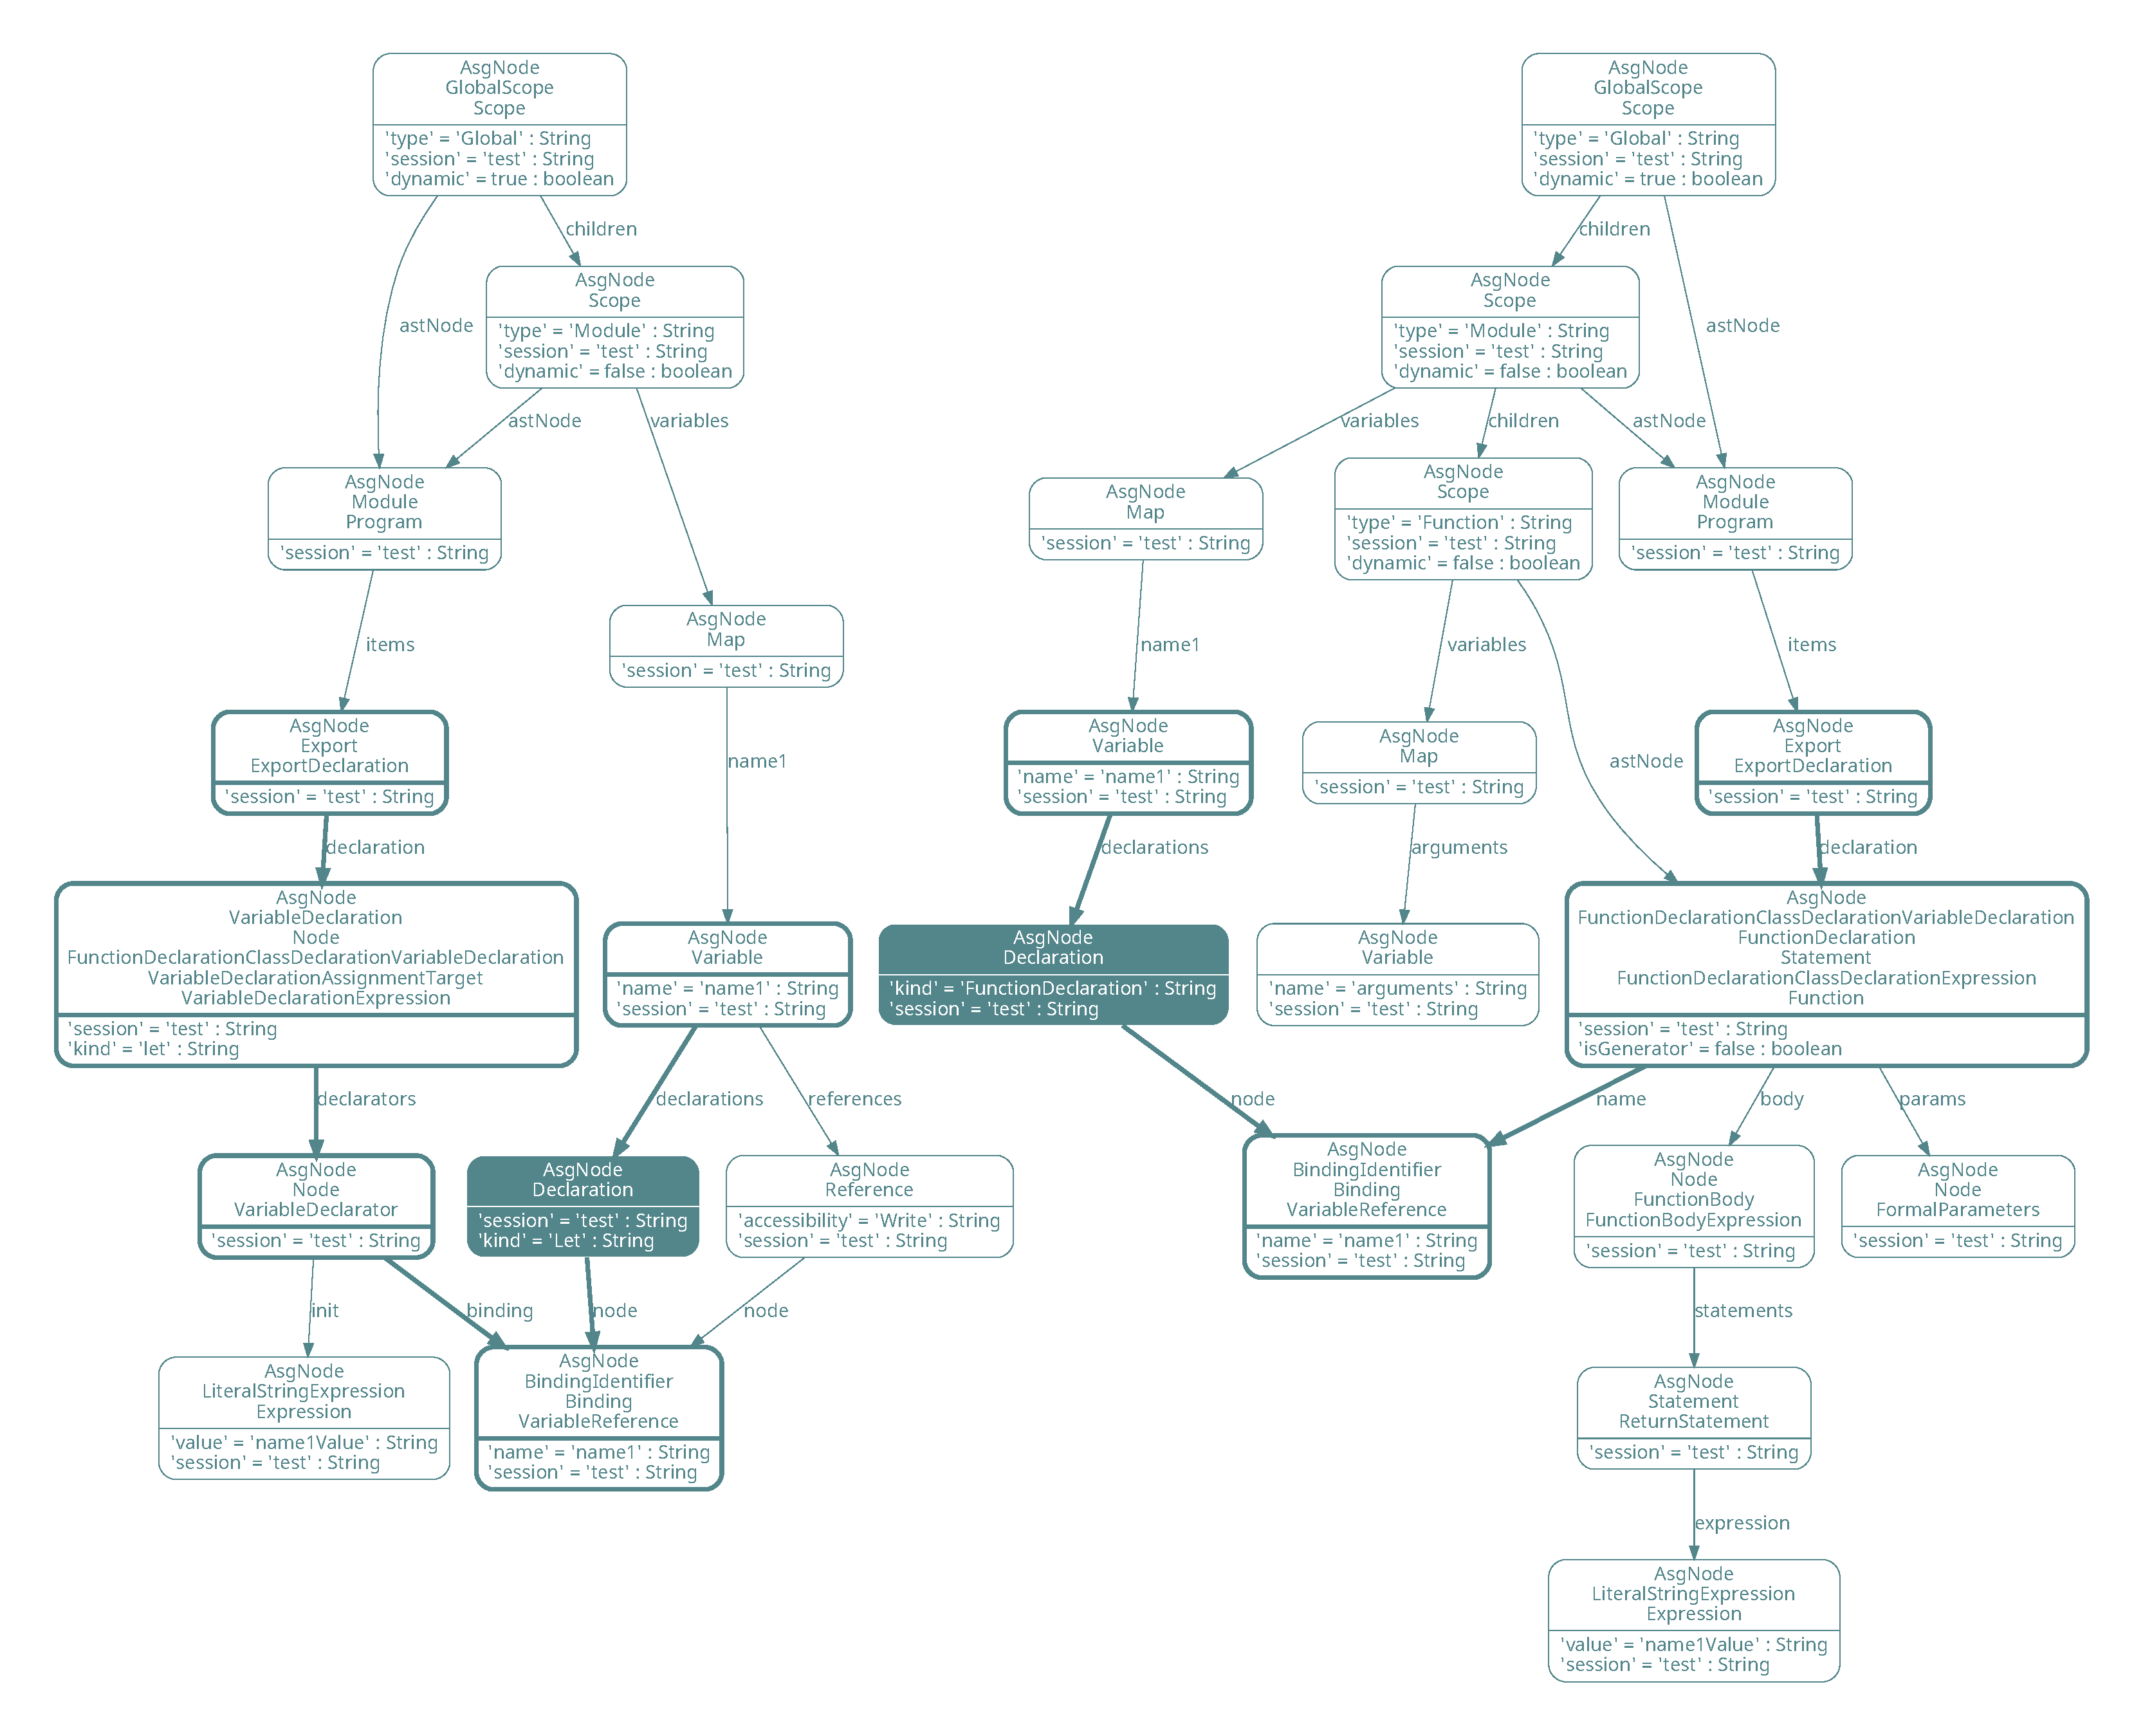
\includegraphics[width=\textwidth, trim=5mm 5mm 5mm 5mm,clip]{figures/export-declaration-demonstration.pdf}
	\caption{Two isomorphic export cases contain the same pattern}
	\label{fig:export-declaration-demonstration}
\end{figure}

The process of pattern generalisation needs to be performed carefully. The generalised patterns must match only those export cases' patterns that can be interconnected with imports in a semantically correct way. If the patterns are too broadly generalised, they will match more export cases than intended, resulting in semantically incorrect interconnections (between incompatible export-import cases). In contrary, if they are too narrowly specified, they will match only one export case, resulting no reduction of the $\alpha$.

In the following, I list all export cases I found to be isomorphic in groups. Each group's name implies why the elements are isomorphic in the group. Since every element can be interconnected with imports using the same algorithm per group, an isomorphic group with its elements can be considered as one generalised export case regarding the ASG interconnection process of the Codemodel-Rifle framework. The following $5$ isomorphic export groups have been formed:

\begin{itemize}
\item \textbf{\lstinline{exportName}}
	\begin{itemize}
	\item \lstinline{exportName}
	\end{itemize}

\item \textbf{\lstinline{exportDefaultName}}
	\begin{itemize}
	\item \lstinline{exportDefaultName}
	\end{itemize}

\item \textbf{\lstinline{exportAlias}}
	\begin{itemize}
	\item \lstinline{exportAlias}
	\item \lstinline{exportAsDefault}
	\end{itemize}

\item \textbf{\lstinline{exportDeclaration}}
	\begin{itemize}
	\item \lstinline{exportEmptyLetDeclaration}
	\item \lstinline{exportEmptyVarDeclaration}
	\item \lstinline{exportLetDeclaration}
	\item \lstinline{exportVarDeclaration}
	\item \lstinline{exportConstDeclaration}
	\item \lstinline{exportClass}
	\item \lstinline{exportFunction}
	\item \lstinline{exportGenerator}
	\end{itemize}

\item \textbf{\lstinline{exportDefaultDeclaration}}
	\begin{itemize}
	\item \lstinline{exportDefaultClass}
	\item \lstinline{exportDefaultFunction}
	\item \lstinline{exportDefaultGenerator}
	\end{itemize}
\end{itemize}

Based on the above, having $5$ isomorphic export groups means that the number of distinctly handled export cases has been reduced to $5$. \Cref{table:updated-compatibility-table} shows the updated compatibility table with export cases grouped by their isomorphism, without listing the unsupported cases. By this time, with excluding incompatible and unsupported cases and applying pattern generalisation techniques, $\alpha$ has been reduced to $13$, meaning only $13$ separate algorithms have to be implemented in order to cover most of the export-import cases.

\begin{table}[!htb]
	\newcommand{\yep}{\tikz\draw[black,fill=black] (0,0) circle (0.8ex);\xspace}
	\newcommand{\nop}{\tikz\draw[black,fill=none] (0,0) circle (0.8ex);\xspace}

	\centering
	\small
	\begin{tabular}{l|ccc}
		\hline
																& \rotatebox{90}{importName}
																& \rotatebox{90}{importAlias}
																& \rotatebox{90}{importDefault~~}
																\\
		\hline
		exportName									& \yep & \yep & \nop \\
		exportDefaultName						& \yep & \yep & \yep \\
		exportAlias									& \yep & \yep & \yep \\
		exportDeclaration						& \yep & \yep & \nop \\
		exportDefaultDeclaration		& \yep & \yep & \yep \\
		\hline
	\end{tabular}

	\caption{Export-import compatibility matrix with exports grouped by their isomorphism}
	\label{table:updated-compatibility-table}
\end{table}


\subsection{Implementing the Interconnection Algorithms}

After thoroughly inspecting the ASG-signatures of the numerous export and import cases for minimising the number of algorithms to be implemented, actually implementing the algorithms was straightforward. In this section, I will not present all cases in detail. Instead, I describe the general steps of the interconnection process, provide a complete example of one concrete case, and describe the algorithms of other cases in the Appendix.

The steps of the interconnection process in general can be described as the following:

\begin{enumerate}
\item Match each to-be-exported entities of the exporter module with strictly unique patterns containing all necessary identifiers and information for the export.
\item Match each to-be-imported entities of the importer module with strictly unique patterns containing all necessary identifiers and information for the import.
\item Perform interconnections between the exporter module and the importer module by finding corresponding entities in the two modules based on identifiers like names and/or default export/import bindings.
\item Clean the graph, so it will not contain duplicate nodes or edges after the interconnection process.
\end{enumerate}

\begin{figure}[!htb]
	\begin{lstlisting}[language=JavaScript]
			// exporter.js
			let name1 = "name1Value";
			export { name1 };

			// importer.js
			import { name1 as importedName1 } from "exporter";
	\end{lstlisting}
  \caption{Modules of the \emph{exportName–importAlias} demonstration}
  \label{fig:export-import-example-source}
\end{figure}

I chose the fully detailed case to be the \emph{exportName–importAlias}. The \emph{exportName} is present in the \lstinline{exporter} module, while the \emph{importAlias} is present in the \lstinline{importer} module. \Cref{fig:export-import-example-source} shows the source code of the two modules.

\Cref{fig:export-import-example-asg} displays the process of interconnecting the \lstinline{exporter} module with the \lstinline{importer} module along the \emph{exportName–importAlias} case. The following steps are necessary in the ASG of the modules:
\begin{enumerate}
\item Find the exported \lstinline{Variable} with its \lstinline{Declaration} in the \lstinline{exporter} module marked with blue colour. The full matched pattern is indicated with thicker outlines.
\item Find the imported \lstinline{Variable} with its \lstinline{BindingIdentifier} and its \lstinline{Declaration} in the \lstinline{importer} module marked with crimson colour. The full matched pattern is indicated with thicker outlines.
\item Check if the \lstinline{Import} node's \lstinline{moduleSpecifier} attribute is equal to the exporter module's name (currently \lstinline{exporter}).
\item Check if the \lstinline{name} attribute of the \lstinline{IdentifierExpression} node (connecting to the \lstinline{ExportLocalSpecifier} node) is equal to the \lstinline{ImportSpecifier} node's \lstinline{name} attribute. In this particular \emph{importAlias} case, checking \lstinline{ImportSpecifier} node's \lstinline{name} attribute instead of the imported \lstinline{Variable} node's \lstinline{name} attribute provides the support for the \emph{aliased} import.
\item Create a \lstinline{declarations} edge from the imported \lstinline{Variable} node to the exported \lstinline{Declaration}. This is indicated with a thick black outline.
\item Create a \lstinline{node} edge from the exported \lstinline{Declaration} node to the imported variable's \lstinline{BindingIdentifier} node. This is indicated with a thick black outline.
\item Delete the original \lstinline{Declaration} node of the imported variable with its edges.\footnote{This step does not cause loss of information: the graph still contains the information that the variable was \emph{imported}.}
\end{enumerate}

These steps are translated to Cypher, and sent to the database. Each export-import combination featured in \Cref{table:updated-compatibility-table} has a separate Cypher query. As these \emph{export-import interconnection queries} are \emph{independent} from each other — they do not modify the others' results in any way — they can be executed in any order. The queries are also \emph{idempotent}: they can be re-executed arbitrarily many times without different outcomes on the same dataset.

\Cref{fig:export-import-example-cypher-source} presents the full Cypher query of the \emph{exportName–importAlias} case featured in the example. The query contains a node with a label that is not displayed in the visualised graph: \lstinline{CompilationUnit}. At translating the modules into ASGs, Codemodel-Rifle creates a node with the label \lstinline{CompilationUnit} for each distinct source file. Each module's all graph nodes is connected to the module's \lstinline{CompilationUnit} node. The node also stores the information about the parsed module's file path. As displaying the \lstinline{CompilationUnit} node and all its connections to all other nodes would make the graph very dense and unclear, it is omitted from the visualisation.

% Floating two figures on two consecutive pages does not work, had to be hacked
\newpage
\vspace*{7em}
\begin{figure}[!h]
	\centering
	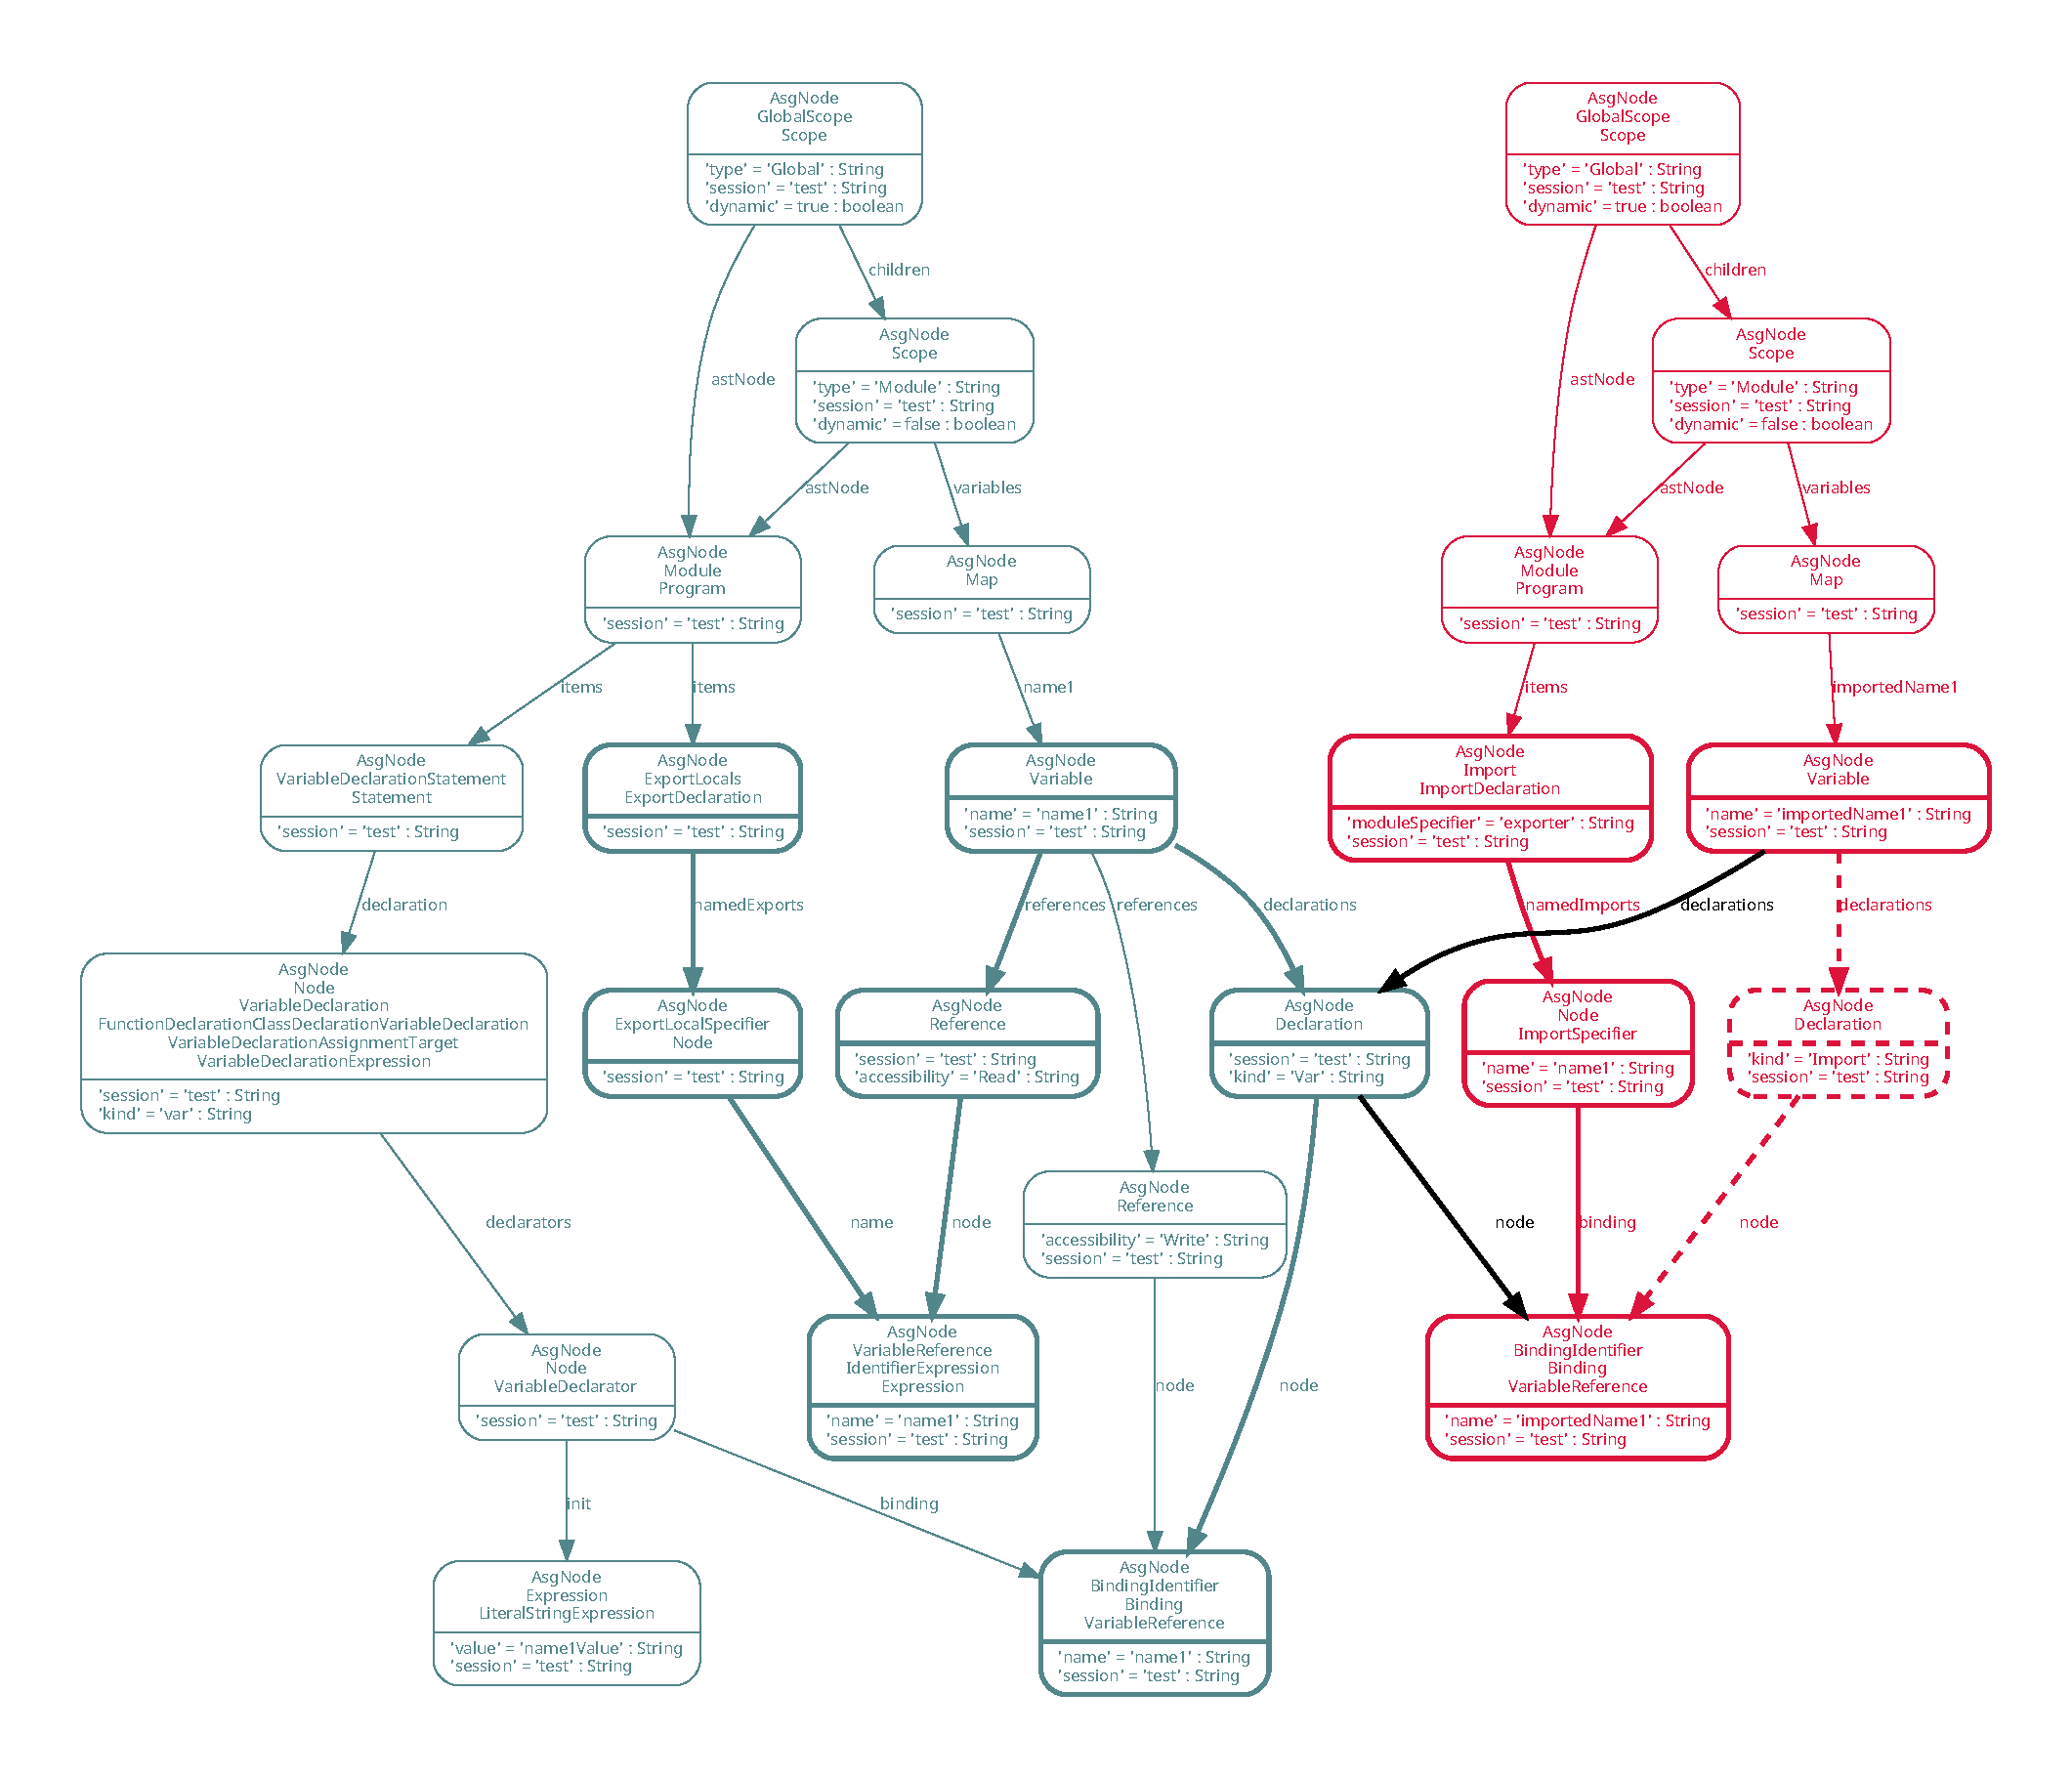
\includegraphics[width=\textwidth, trim=5mm 5mm 5mm 5mm,clip]{figures/export-import-example-asg.pdf}
	\caption{Interconnecting the \lstinline{exporter} module with the \lstinline{importer} module in the case \emph{exportName–importAlias}}
	\label{fig:export-import-example-asg}
\end{figure}

% Floating two figures on two consecutive pages does not work, had to be hacked
\newpage
\vspace*{5.3em}
\begin{figure}[!h]
	\begin{lstlisting}[language=Cypher]
MATCH
// exporter.js: let name1 = "name1Value"; export { name1 };
    (exporter:CompilationUnit)-[:contains]->(:ExportLocals)
        -[:namedExports]->(:ExportLocalSpecifier)
        -[:name]->(exportBindingIdentifier:IdentifierExpression)
        <-[:node]-(:Reference)
        <-[:references]-(:Variable)
        -[:declarations]->(declarationToMerge:Declaration)
        -[:node]->(:BindingIdentifier),

// importer.js: import { name1 as importedName1 } from "exporter";
    (importer:CompilationUnit)-[:contains]->(import:Import)
        -[:namedImports]->(importSpecifier:ImportSpecifier)
        -[:binding]->(importBindingIdentifierToMerge:BindingIdentifier)
        <-[:node]-(declarationToDelete:Declaration)
        <-[:declarations]-(importedVariable:Variable)

    WHERE
    exporter.parsedFilePath CONTAINS import.moduleSpecifier
    AND exportBindingIdentifier.name = importSpecifier.name

CREATE UNIQUE
    (importedVariable)-[:declarations]->(declarationToMerge),
    (declarationToMerge)-[:node]->(importBindingIdentifierToMerge)

DETACH DELETE
    declarationToDelete
	\end{lstlisting}
  \caption{The Cypher query of the \emph{exportName–importAlias} case}
  \label{fig:export-import-example-cypher-source}
\end{figure}


\newpage
\section{The Qualifier System}


\section{Implementing the Analyses}
